\documentclass{beamer}
\usepackage[utf8]{inputenc}
\usepackage[english,german]{babel} 
\usepackage{listings} 
\usepackage{listings-golang}
\usepackage{tikz}

\usepackage[absolute,overlay]{textpos}
  \setlength{\TPHorizModule}{1mm}
  \setlength{\TPVertModule}{1mm}

\titlegraphic{
\includegraphics[scale=0.3]{logoHaw.png}}
\title{
	\textit{BW2 Praktikum} \\
	\textbf{\\ \"Ubungsblatt 2 - Gruppe 1}
}
\author{Adrian Helberg \\ Version 1.0}
\date{\today}

\definecolor{mygreen}{rgb}{0,0.6,0}

\begin{document}
\lstset{
    frame=single,
    basicstyle=\footnotesize,
    keywordstyle=\color{blue},
    showstringspaces=false, 
    stringstyle=\color{mygreen},
    tabsize=4,
    language=Golang
}

\maketitle

\section{Aufgabe 2}
\begin{frame}
\frametitle{Aufgabe 2}

\begin{quote}
Begleitende Dokumentation
\end{quote}

Der Prozess wird mit der Erweiterten Ereignisgesteuerten Prozesskette (eEPK)  mit dem Webtool ''Signavio Academic'' modelliert.
\begin{itemize}
\item Eindeutigkeit
\item Einfachheit 
\item Leichte Verständlichkeit
\end{itemize}

\end{frame}

\begin{frame}
\frametitle{Aufgabe 2}

Wichtigste Modellierungsentscheidungen:
\begin{itemize}
\item Einfl\"usse durch gewisse Abteilungen, Personen, Systeme und Dokumente werden zu einer Funktion durch eintreffende Pfeile zugeordnet
	\begin{itemize}
	\item Leichtes Zuordnen von Input, Verarbeitung und Output der Sub-Systeme
	\item Kante nicht begehbar, da der eintreffende Pfeil die Zuordnung zeigt
	\item Klare Zust\"andigkeiten
	\item Informationsquellen
	\end{itemize}
\item Farbwahl
	\begin{itemize}
	\item Geld f\"ur Abteilungen / Abteilungsperson
	\item Lila f\"ur Ereignisse
	\item Gr\"un f\"ur Funktionen
	\end{itemize}
\end{itemize}

%\begin{figure}
%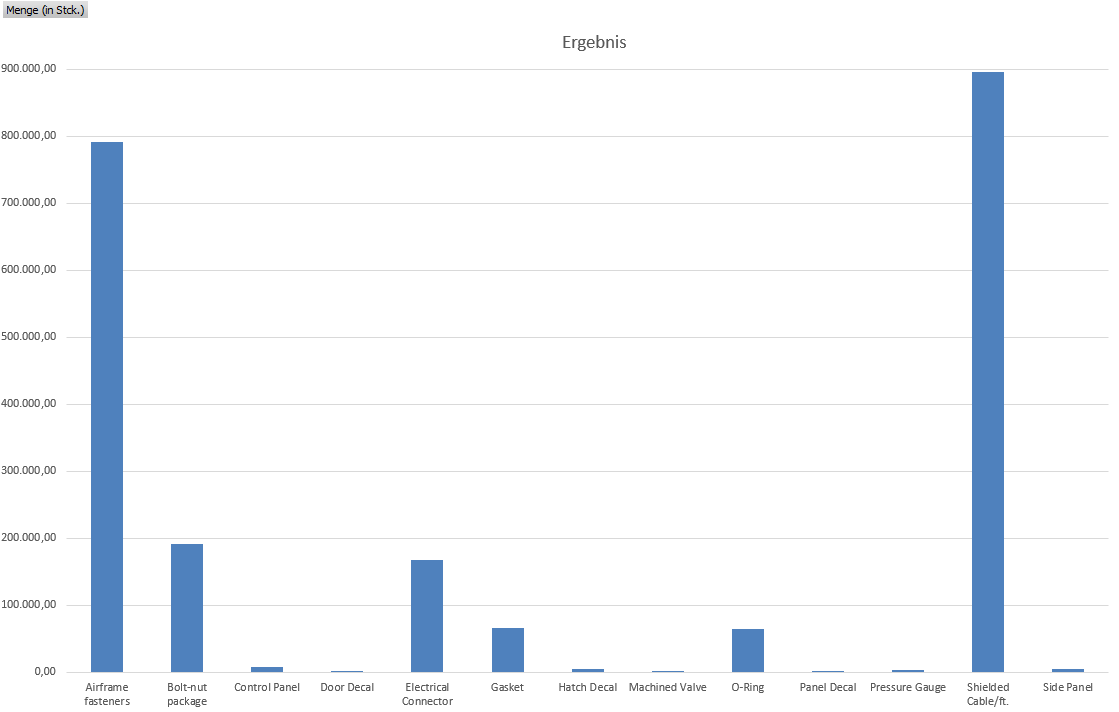
\includegraphics[scale=0.34]{pivot_itemNO_quantity.PNG}
%\end{figure}

\end{frame}

\end{document}